\section{Pianificazione}
\label{Pianificazione}
Basandosi sulle scadenze esposte nella tabella \ref{table:Scadenze} si è deciso di sviluppare il progetto suddividendolo sulla base dello standard ISO/IEC 12207:1995, che prevede le seguenti fasi:
\begin{itemize}
	\item Attività preliminari di Avvio ed Analisi dei Requisiti;
	\item Progettazione\glossario Architetturale;
	\item Progettazione di Dettaglio e Codifica;
	\item Validazione e Collaudo.
\end{itemize}

\begin{longtable}{|C{.46\textwidth}|C{.20\textwidth}|C{.20\textwidth}|}
\hline
\rowcolor{bluelogo}\textbf{\textcolor{white}{Fase}} & \textbf{\textcolor{white}{Inizio}} & \textbf{\textcolor{white}{Fine}}
\\
\hline \hline
\endfirsthead
\hline
Avvio ed Analisi Requisiti & 2018-11-15 & 2019-01-12 \\
\hline
\rowcolor{grigio}\textit{Risanamento Criticità} & 2019-01-22 & 2019-01-25 \\
\hline
Progettazione Architetturale & 2019-01-26 & 2019-03-08 \\
\hline
\rowcolor{grigio}\textit{Risanamento Criticità} & 2019-03-16 & 2019-03-18 \\
\hline
Progettazione di Dettaglio e Codifica & 2019-03-19 & 2019-04-12 \\
\hline
\rowcolor{grigio}\textit{Risanamento Criticità} & 2019-04-20 & 2019-04-22 \\
\hline
Validazione e Collaudo & 2019-04-23 & 2019-05-10 \\
\hline
\caption{Principali Fasi di Sviluppo \label{Tabella Fasi di Sviluppo}}
\end{longtable}

La prima fase sarà a carico del gruppo \texttt{Agents of S.W.E.} mentre le ulteriori fasi saranno a carico del committente. \\
Nonostante la scelta di adottare lo standard ISO/IEC, si è deciso di aggiungere un incremento tra ognuna delle quattro fasi, che consiste in un periodo di sanazione delle criticità trovate dopo un'attenta analisi dell'incremento effettuato, che avviene non solo da parte del gruppo \texttt{Agents of S.W.E.}, ma anche da parte della proponente. 

\subsection{Attività Preliminari di Avvio ed Analisi dei Requisiti}
\label{Apaar}

Il periodo di \textit{Avvio ed Analisi dei Requisiti} va dal 2018-11-15, data di formazione dei gruppi, e termina il 2019-01-14 con la consegna della documentazione relativa alla RR.

\newpage
\subsubsection{Incrementi}

Il primo periodo prevede 6 incrementi e le principali operazioni svolte sono: 
\begin{itemize}
	\item \textbf{\textit{Analisi dei Requisiti v1.0.0}}: all'interno del documento \textit{Analisi dei Requisiti v1.0.0} vengono inseriti tutti i requisiti individuati dagli \textit{Analisti}, analizzando il capitolato d'appalto. Questa risulta essere un'attività particolarmente importante, poiché l'errata analisi comporterebbe un impedimento nell'avanzamento del progetto.
	\item \textbf{\textit{Glossario v1.0.0}}: il documento \textit{Glossario v1.0.0} racchiuderà tutti i termini ambigui o poco chiari che vengono individuati durante la redazione dei documenti;
	\item \textbf{\textit{Lettera di Presentazione}}: l'attività prevede la stesura della \textit{Lettera di Presentazione} dichiarando il gruppo \texttt{Agents of S.W.E.} come fornitore;
	\item \textbf{\textit{Norme di Progetto v1.0.0}}: tutte le norme che vengono stabilite, saranno inserite all'interno del documento \textit{Norme di Progetto v1.0.0} individuate dall'\textit{Amministratore}. Ha lo scopo di uniformare le modalità di lavoro che dovranno essere attuate da tutti i membri del gruppo. Consiste in un'attività critica in quanto fondamentali per la stesura della documentazione;
	
	\item \textbf{\textit{Piano di Progetto v1.0.0}}: è compito del \textit{Responsabile} analizzare attività e scadenze al fine di ottenere una buona riuscita del progetto ed è compito dell'\textit{Amministratore} analizzare i rischi nei quali si può incorrere. Le attività e le risorse vengono suddivise per l'intera durata del progetto ed inserite all'interno del documento \textit{Piano di Progetto v1.0.0}, necessario e vincolante per la stesura della \textit{Lettera di Presentazione};
	\item \textbf{\textit{Piano di Qualifica v1.0.0}}: i \textit{Progettisti} avranno il compito di cercare un elenco di attività e metodi utili al fine di garantire una buona qualità di prodotto. Questi verranno racchiusi all'interno del documento \textit{Piano di Qualifica v1.0.0};
	\item \textbf{\textit{Studio di Fattibilità v1.0.0}}: consiste nell'analisi preliminare dei vari capitolati proposti ed è essenziale alla fine della scelta del capitolato da svolgere. L'analisi verrà inserita all'interno del documento \textit{Studio di Fattibilità v1.0.0}; questa risulta essere un'attività bloccante per l'inizio dell'attività di Analisi dei Requisiti.  
\end{itemize}
\newpage
\begin{landscape}
\subsubsection{Diagramma di Gantt}
\begin{figure}[H]
	\centering
  		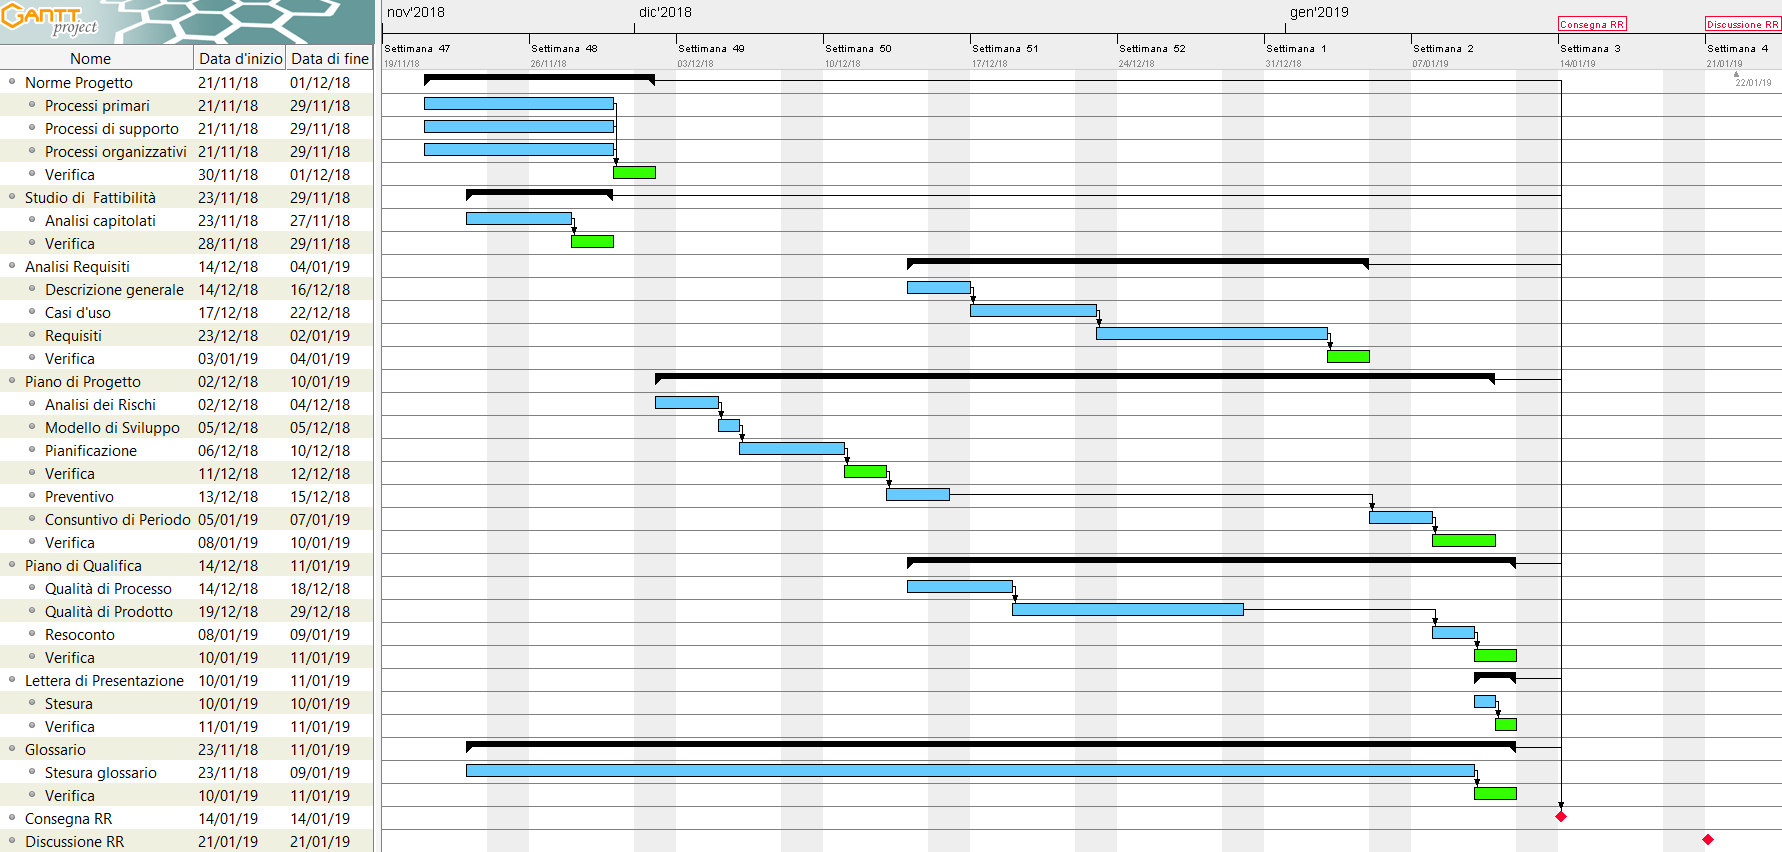
\includegraphics[width=1.0\linewidth]{./images/AvvioAnalisi.png}
  		\caption{Diagramma di Gantt per Attività di Avvio ed Analisi}
  		\label{fig:Gantt Avvio ed Analisi}
\end{figure}
\end{landscape}
\newpage


\subsection{Risanamento Criticità}
\label{RC1}

Con \textit{Risanamento delle Criticità}, fase all'infuori dello standard ISO, si intende un periodo prefissato, in cui si andrà ad analizzare le varie criticità che sono emerse alla fine dei vari incrementi, dopo la loro analisi sia da parte della proponente che da parte del gruppo. \\
Nel caso in cui il tempo preventivato per questa fase dovesse risultare superiore a quello effettivamente richiesto, le ore in eccesso verranno utilizzate per l'incremento successivo.\\
La scelta di inserire questo tra la prima e la seconda fase è guidata dal fatto che per procedere è necessario aver risolto tutti i problemi riscontrati nelle produzioni precedenti, in particolar modo la seconda fase, individuata dallo standard, prevede la \textit{Progettazione Architetturale} ed è quindi fondamentale sanare i problemi sorti nel primo periodo. 
Il primo periodo di \textit{Risanamento delle Criticità} si svolgerà dal 2019-01-22 al 2019-01-25  e si avrà un solo incremento.

\subsubsection{Diagramma di Gantt}

\begin{figure}[h]
	\centering
  		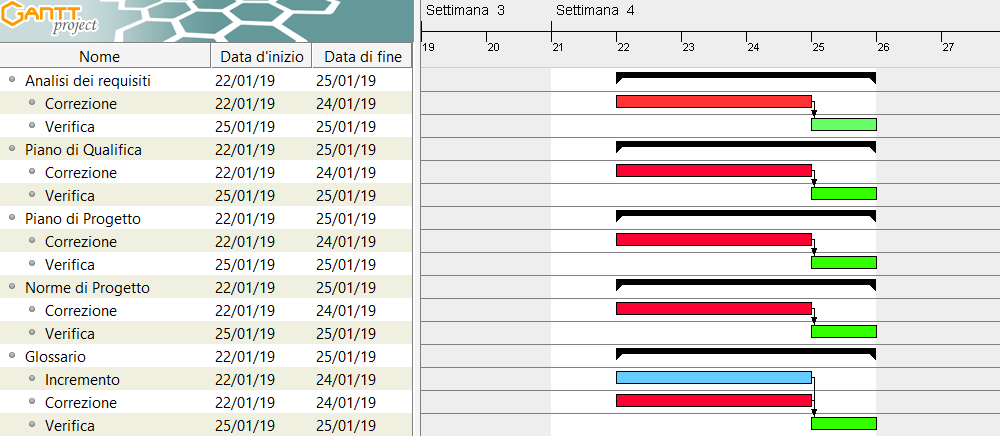
\includegraphics[width=1.0\linewidth]{./images/RisanamentoCriticita1.png}
  		\caption{Diagramma di Gantt per Attività Risanamento delle Criticità Parte 1}
  		\label{fig:Gantt Risananmento Criticità 1}
\end{figure}

\newpage
\subsection{Progettazione Architetturale}
\label{PA}

Il periodo di \textit{Progettazione Architetturale} inizia dalla fine del periodo di \textit{Risanamento Criticità} e termina con la consegna del nuovo incremento (quindi dal 2019-01-26 al 2019-03-08), il quale prevede le operazioni riportate nella sottosezione seguente.

\subsubsection{Incrementi}

Il seguente periodo prevede 4 incrementi, durante i quali verranno svolte le seguenti attività:

\begin{itemize}
	\item \textbf{Incremento e Verifica}: all'inizio del periodo vengono svolte attività di incremento e verifica su vari documenti (\textit{Norme di Progetto v2.0.0, Piano di Progetto v2.0.0, Piano di Qualifica v2.0.0});
	\item \textbf{Studio Tecnologie}: prevede un continuo approfondimento delle tecnologie necessarie allo svolgimento del progetto; 
	\item \textbf{Technology Baseline}\glossario: questa attività prevede l'analisi e la scelta di tecnologie, framework\glossario e librerie\glossario da utilizzare. In questa fase, inoltre, è previsto lo sviluppo del \textit{Proof of Concept}\glossario;
	\item \textbf{\textit{Glossario v2.0.0}}: aggiunta e modifica dei termini in itinere;  
	\item \textbf{Verifica}\glossario: cinque giorni prima della fine del periodo sarà compito dei \textit{Verificatori} analizzare i risultati della seconda fase segnalando, a chi di dovere, gli errori o le imprecisioni riscontrate.
\end{itemize}

\begin{landscape}
\subsubsection{Diagramma di Gantt}
\begin{figure}[h]
	\centering
  		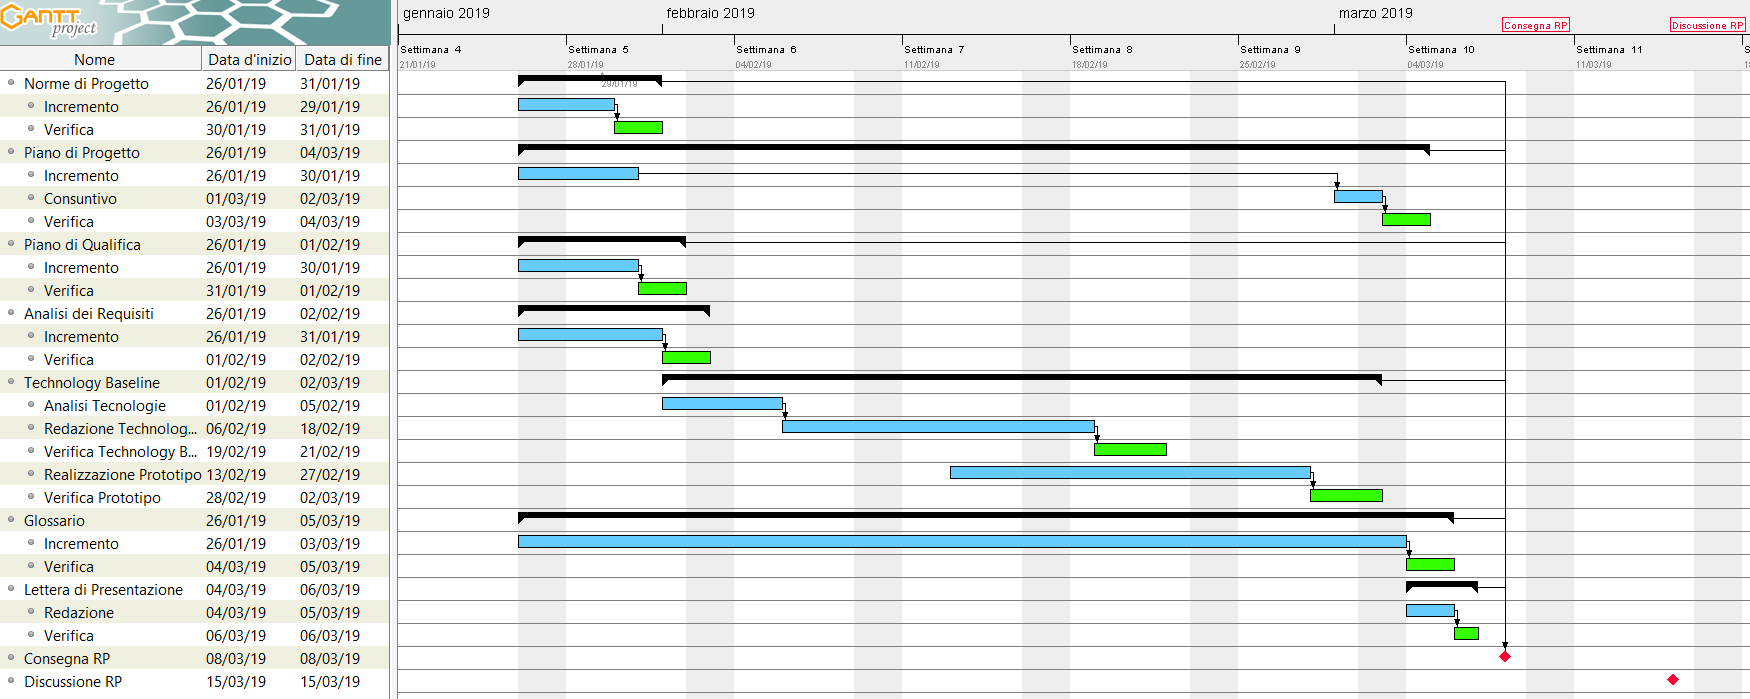
\includegraphics[width=1.0\linewidth]{./images/ProgettazioneArchitetturale.png}
  		\caption{Diagramma di Gantt per Attività di Progettazione Architetturale}
  		\label{fig:Gantt Progettazione Architetturale}
\end{figure}
\end{landscape}

\subsection{Risanamento Criticità}
\label{RC2}
In questo periodo di \textit{Risanamento delle Criticità}, andremo a risolvere i restanti problemi dalla prima fase(qualora ve ne fossero ancora). Inoltre, aggiusteremo i problemi riscontrati nella fase di \textit{Progettazione Architetturale} relativi a \textit{Technology Baseline} e \textit{Proof of Concept} in vista dei prossimi incrementi.
Il secondo periodo di \textit{Risanamento delle Criticità} andrà dal 2019-03-16 al 2019-03-18 e verrà effettuato un solo incremento.

\subsubsection{Diagramma di Gantt}

\begin{figure}[h]
	\centering
  		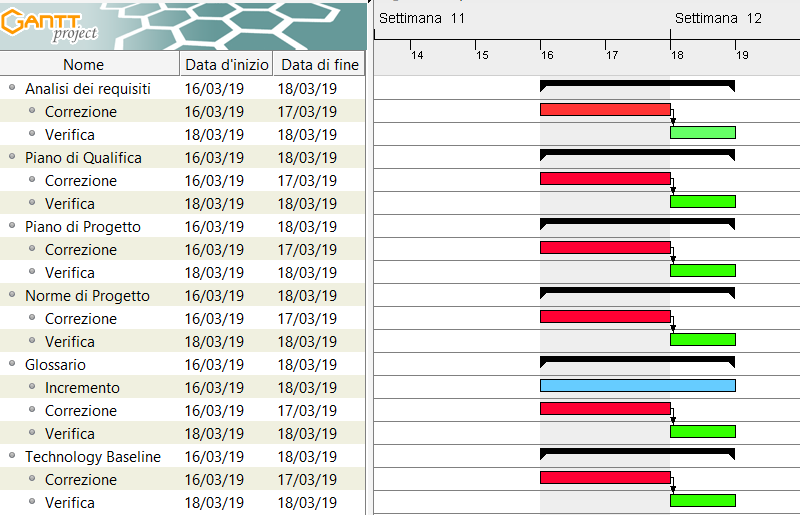
\includegraphics[width=1.0\linewidth]{./images/RisanamentoCriticita2.png}
  		\caption{Diagramma di Gantt per Attività Risanamento delle Criticità Parte 2}
  		\label{fig:Gantt Risananmento Criticità 2}
\end{figure}

\newpage
\subsection{Progettazione di Dettaglio e Codifica}
\label{PDC}
Il periodo di \textit{Progettazione di Dettaglio e Codifica} va dal giorno dopo la fine del periodo di \textit{Risanamento delle Criticità}, cioè il 2019-03-19, e termina con la consegna dei documenti per la RQ, cioè il 2019-04-12.\\

\subsubsection{Incrementi}
Il seguente periodo prevede 3 incrementi, durante i quali verranno svolte le seguenti attività:
\begin{itemize}
	\item \textbf{Incremento e Verifica}: all'inizio del periodo vengono svolte attività di incremento e verifica su vari documenti (\textit{Norme di Progetto v3.0.0, Piano di Progetto v3.0.0, Piano di Qualifica v3.0.0 e Technology Baseline});
	\item \textbf{\textit{Glossario v3.0.0}}: prevede l'aggiunta di nuovi termini al \textit{Glossario v3.0.0} ed il suo miglioramento;
	\item \textbf{Product Baseline}\glossario: presenta la baseline\glossario architetturale del prodotto, coerente rispetto a quanto riportato nella \textit{Technology Baseline}. Al suo interno contiene i diagrammi delle classi e di sequenza, la contestualizzazione dei design pattern adottati nell'architettura del prodotto; 
	\item \textbf{Codifica}: prevede la scrittura del codice e relativa verifica di esso;
	\item \textbf{\textit{Manuale Utente v1.0.0}}: consiste nella redazione del \textit{Manuale Utente v1.0.0}, contenente le indicazioni d'utilizzo del prodotto;
	\item \textbf{\textit{Lettera di Presentazione}}: prevede la stesura della \textit{Lettera di Presentazione} per la partecipazione alla RQ.
\end{itemize}


\begin{landscape}
\subsubsection{Diagramma di Gantt}
\begin{figure}[h]
	\centering
  		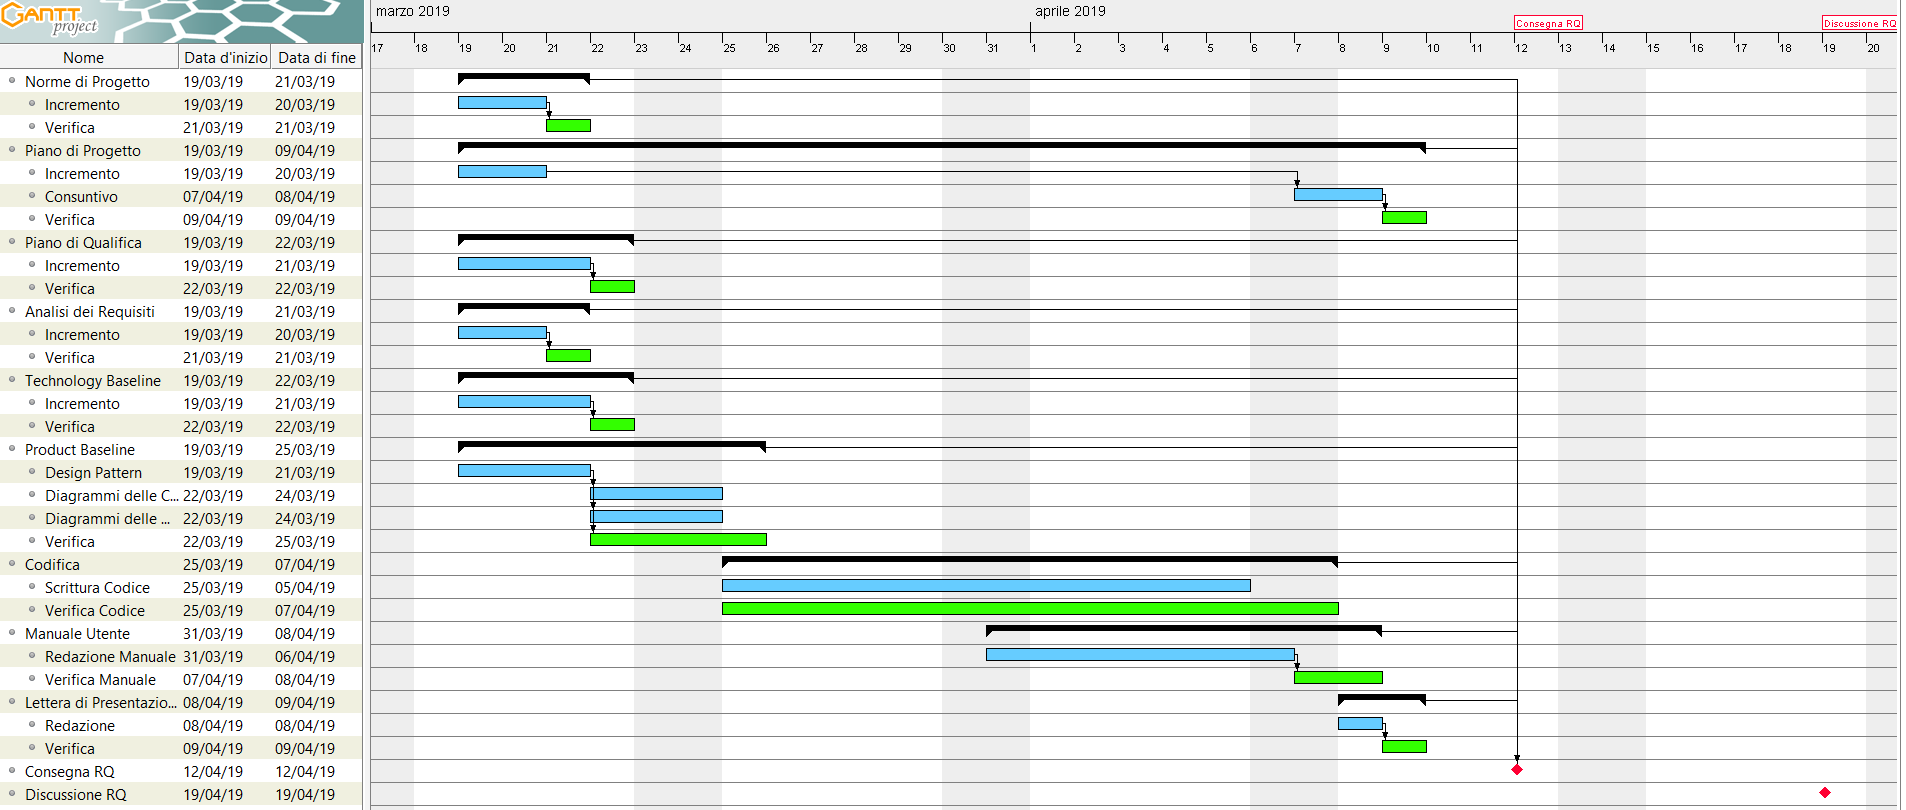
\includegraphics[width=1.0\linewidth]{./images/DettaglioeCodifica.png}
  		\caption{Diagramma di Gantt per Attività di Progettazione di Dettaglio e Codifica}
  		\label{fig:Gantt Progettazione di dettaglio e codifica}
\end{figure}
\end{landscape}

\subsection{Risanamento Criticità}
\label{RC3}
In questo periodo di \textit{Risanamento delle Criticità}, andremo a risolvere i restanti problemi dalla terza fase. Inoltre, aggiusteremo i problemi riscontrati nella fase di \textit{Progettazione di Dettaglio e Codifica} relativi a \textit{Product Baseline} e \textit{Manuale Utente v1.0.0} in vista dei prossimi incrementi.
Il terzo periodo di \textit{Risanamento delle Criticità} andrà dal 2019-04-20 al 2019-04-22; verrà effettuato un solo incremento.

\subsubsection{Diagramma di Gantt}
\begin{figure}[h]
	\centering
  		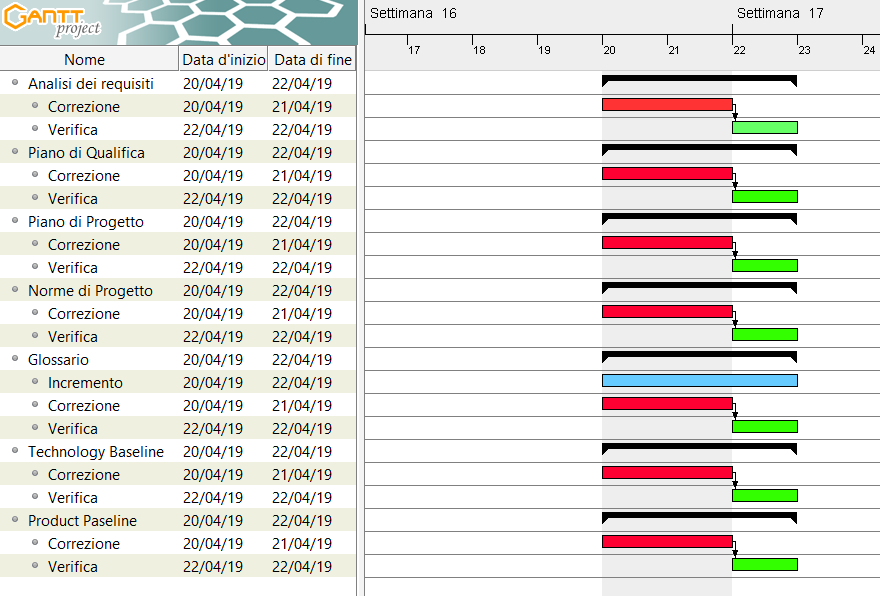
\includegraphics[width=1.0\linewidth]{./images/RisanamentoCriticita3.png}
  		\caption{Diagramma di Gantt per Attività Risanamento delle Criticità Parte 3}
  		\label{fig:Gantt Risananmento Criticità 3}
\end{figure}

\newpage
\subsection{Validazione e Collaudo}
\label{VEC}
Il periodo di \textit{Validazione e Collaudo} inizia il 2019-04-23 e termina il 2019-05-10 con la consegna dei documenti per la RA. 


\subsubsection{Incrementi}
Il seguente periodo prevede 2 incrementi, durante i quali verranno svolte le seguenti attività:
\begin{itemize}
	\item \textbf{Incremento e Verifica}: all'inizio del periodo vengono svolte attività di incremento e verifica su vari documenti (\textit{Norme di Progetto v4.0.0, Piano di Progetto v4.0.0, Piano di Qualifica v4.0.0 e Technology Baseline});
	\item \textbf{\textit{Glossario v4.0.0}}: prevede l'aggiunta di nuovi termini al \textit{Glossario v4.0.0} ed il suo miglioramento;
	\item \textbf{Validazione e Collaudo}: prevede lo sviluppo ultimo del prodotto, inserendovi miglioramenti e svolgendo ulteriori test, al fine di assicurare e completare il completo soddisfacimento dei requisiti;
	\item \textbf{\textit{Manuale Utente v2.0.0}}: prevede il miglioramento e completamento del \textit{Manuale Utente v2.0.0}, contenente le indicazioni di utilizzo del prodotto.
\end{itemize}

\begin{landscape}
\subsubsection{Diagramma di Gantt}
\begin{figure}[H]
	\centering
  		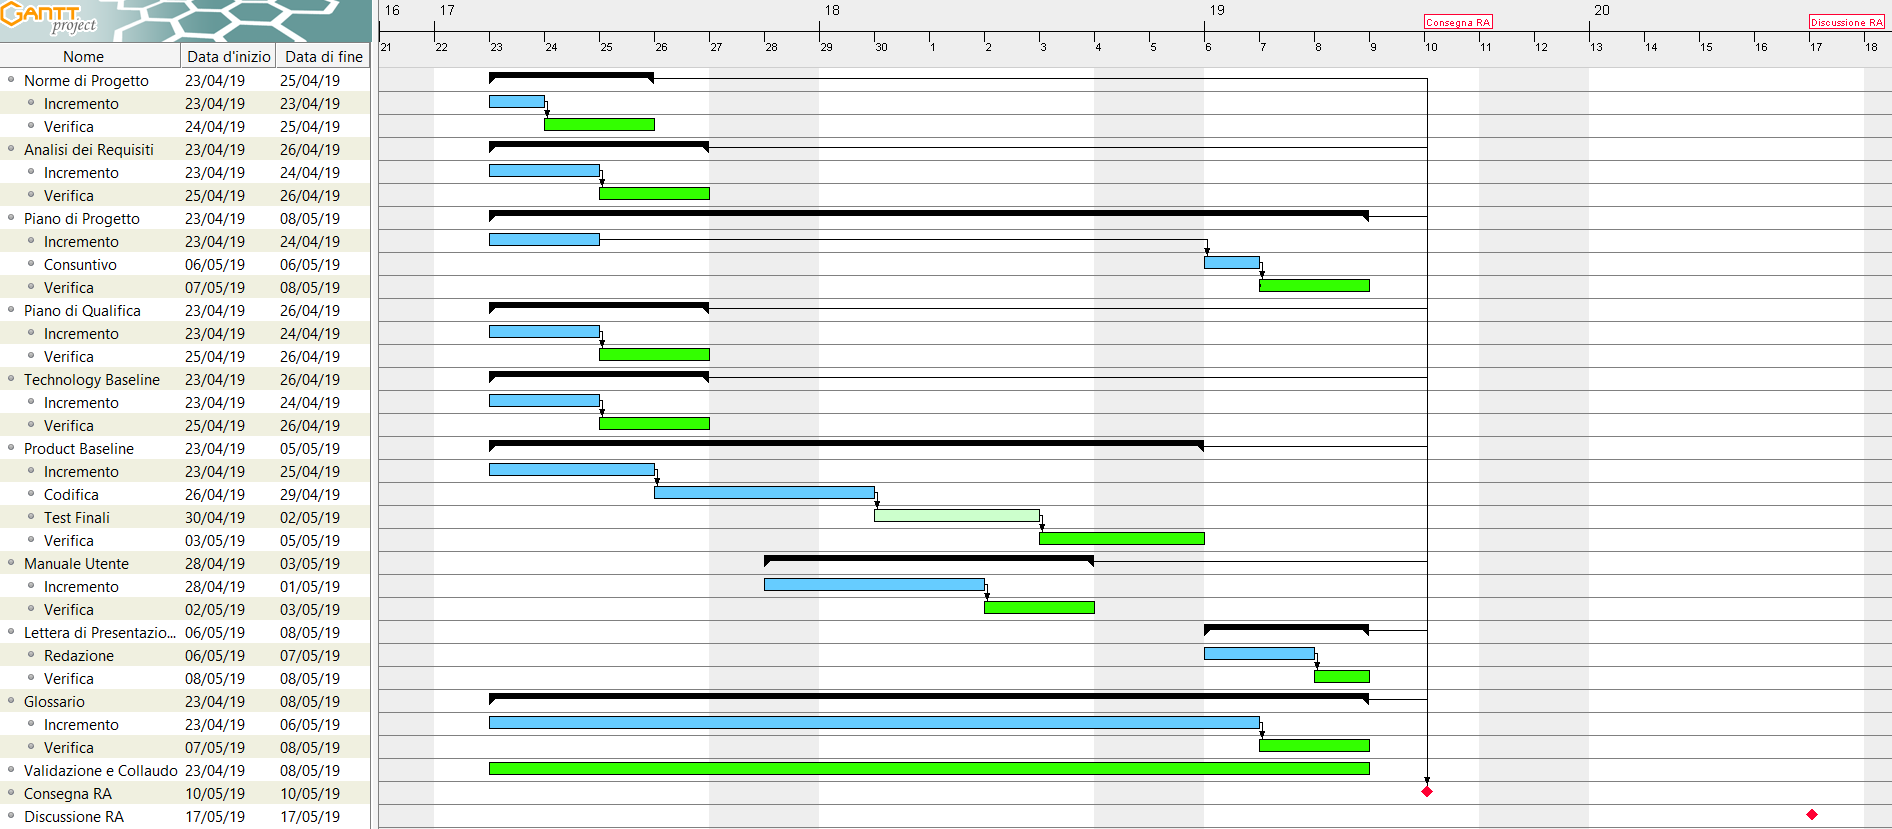
\includegraphics[width=1.0\linewidth]{./images/ValidazioneeCollaudo.png}
  		\caption{Diagramma di Gantt per Attività di Validazione e Collaudo}
  		\label{fig:Gantt Validazione e Collaudo}
\end{figure}
\end{landscape}